\section{The Benchmark - droidXP}

\begin{figure*}[ht]
  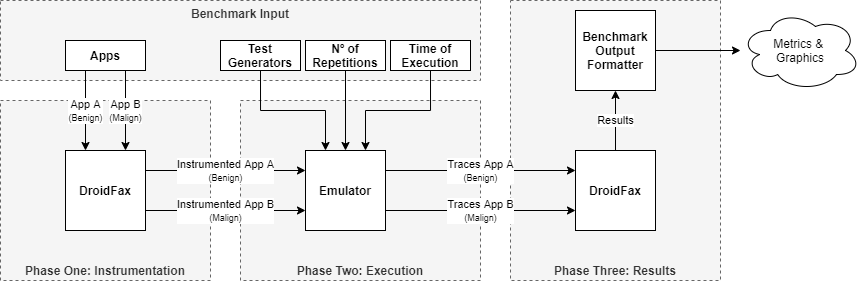
\includegraphics[width=1\textwidth]{images/benchmark3.png}
  \label{benchArq}
  \caption{Benchmark architecture}
  \label{fig:benchArq}
\end{figure*}


To systematically assess and compare test generation tools for mining android sandboxes, we use a benchmark solution, called DroidXP. It relies on a simple \emph{Command Line Interface} (CLI) that favors the execution and configuration of the benchmark. It also
relies on DroidFax \cite{cai2016understanding}, a tools that instruments Android apps and collects relevant information about their execution, like the set of sensitive APIs a given
app calls during a test execution. DroidFax also collects inter-component communication (ICC)  intent  tracing  using  static  program analysis.

The droidXP CLI provides two commands: a command that lists all test case
generation tools (executing the project with the option ``list-tools'') that had been
integrated into the benchmark; and a command that performs the execution of the benchmark,
which can be configured using the following parameters:

\begin{itemize}
    \item \texttt{-tools}: Specifies the test tools used in the experiment
    \item \texttt{-t}: Specifies the threshold (in seconds) for the execution time in the experiment
    \item \texttt{-r}: Specifies the number of repetitions used in the experiment
    \item \texttt{-output-format}: Specifies the output format
    \item \texttt{--debug}: Specifies to run in DEBUG mode (default: false)    
\end{itemize}

The droidXP architecture relies on the pipes-and-filters architectural style \cite{architecture-book} (Figure \ref{fig:benchArq}),
and includes three main components; where each component is responsible for a specific phase of the
benchmark (instrumentation, execution, and result analysis).

\subsection{Phase 1: Instrumentation}

In the first phase, a researcher must define the corpus of APK files droidXP
should consider during a benchmark execution. After that, droidXP starts the DroidFax service that instruments each APK file, so that droidXP would be able to collect data about each execution. To improve the performance of the benchmark, the instrumentation phase runs only once for each APK. In this phase, the DroidFax tool also runs some static analysis procedures, to collect the number of methods and classes of each app, which is a necessary information to estimate code coverage.

\subsection{Phase 2: Execution}

In this phase, droidXP installs an (already instrumented) APK file into
an Android emulator, and then executes a test case generation tool
during a period of time. This process repeats for every test case generation
tool and APK files. To provide repeatability of the experiment,
droidXP removes all data stored in the emulator before starting
a new execution. That is, every execution uses a \emph{fresh} emulator,
without any information that might have been kept during
previous executions. 

The benchmark is relatively easy to add new test
case generation tools. To achieve this goal, it leverage the
Strategy Design pattern \cite{patterns-book}, which sets a contract between a family of classes that, in our case, abstracts the specificities for running each tool we want to integrate into droidXP. Listing \ref{lst:toolspec} shows the contract a developer must override to integrate a new tool. According to this contract, one have to: (a) implement a class that inherits from \texttt{ToolSpec}, define constructors that calls the \texttt{super} constructor, passing the name, the description, and the process id as arguments, and (c) implement the \texttt{execute} method, which receives as argument the path of an APK file and a timeout. 

%\begin{lstlisting}[caption=ToolSpec Sample, language=Python, label={lst:toolspec}, basicstyle=\tiny]
\begin{lstlisting}[caption=ToolSpec Sample,label={lst:toolspec}]
class ToolSpec(AbstractTool):
  def __init__(self):
    super(ToolSpec, self).__init__(
      "Test Generator Name", 
      "Test Generator Description", 
      "process_id"
    )
        
  def execute(self, path, timeout):
    # Execute test generator ...
\end{lstlisting}

The benchmark uses the last parameter to kill the execution process
on the emulator after a \emph{timeout event} throws.
This step is necessary to provide a fresh environment
for the next test execution. The actual logic for executing a
specific tool resides in the  \texttt{execute} method,
so it is the responsibility of a developer to
set up all configuration necessary to run a specific
test case generation tool. To performance our study replication we integrated successfully 
the following tools into droidXP. 

\begin{enumerate}[(a)]
  \item {\bf Monkey} is a Google testing utility that generates
    pseudo-random streams of user events. 
    \item {\bf DroidBot}  is a test input generator for
       Android, which sends random or scripted input events~\cite{li2017droidbot}. 
    \item {\bf DroidMate} is an automated execution generator /
      dynamic analysis engine for Android apps\cite{jamrozik2016droidmate}. 
      generation for Android~\cite{mao2016sapienz}. 
    \item {\bf Humanoid} is a tool that uses deep learning techniques to explore Android apps, mimicking the human behavior\cite{li2019deep}; 
    \item {\bf Joke} is a make-believe tool that perform no analysis dynamic, and execute just the static analysis from droifax. More detail about this fake tool will be discussed in the next section; 
\end{enumerate}

\subsection{Phase 3: Result Analysis}

During the execution, all the data that is required to compute the results are provided by Logcat \cite{Logcat}, one of the Android SDK's native tools and is a command-line tool that dumps a log from the Android emulator. Thus, the only part of the log that is analyzed in this phase is the messages sent by the methods inside the Android app that were instrumented on the first phase using the DroidFax tool. 

Droidfax computes the coverage each test achieved and which sensitive API was accessed during the execution of that test. That last information is required to compute the test generator performance in identifying malicious apps by spotting differences between the sensitive API accessed by each version of an app. This information is vital to the measurement of the test generator performance and qualification. After this phase, the benchmark outputs the results of the experiment, which is informing the performance of one or more testing generator tools in mining sandboxes.
